\documentclass[11pt]{article}

% --- packages (all available on Overleaf by default) -----------------------------------------
\usepackage[a4paper,margin=1in]{geometry}
\usepackage{amsmath,amssymb}
\usepackage{graphicx}
\usepackage{booktabs}
\usepackage{array}
\usepackage{xcolor}
\usepackage[hidelinks]{hyperref}
\usepackage[round]{natbib}
\usepackage{algorithm}
\usepackage{algpseudocode}
\usepackage{tikz}
\usetikzlibrary{shapes.geometric,arrows.meta,positioning,calc,fit}

% simple TikZ node styles for the flowchart / activity diagram
\tikzstyle{proc}=[rectangle,rounded corners,draw,align=center,fill=blue!5,minimum height=8mm,text width=34mm,font=\small]
\tikzstyle{sig}=[rectangle,draw,align=center,fill=green!6,minimum height=8mm,text width=32mm,font=\small]
\tikzstyle{dec}=[diamond,aspect=2,draw,align=center,fill=orange!12,inner sep=1pt,font=\small,text width=22mm]
\tikzstyle{term}=[rectangle,rounded corners=10pt,draw,align=center,fill=gray!8,minimum height=8mm,text width=34mm,font=\small]
\tikzstyle{fl}=[-{Stealth[length=2mm]},thick]

\title{\textbf{CADIS: A Consequence-Aware Dynamic Intervention System\\ for Overseeing LLM Penetration-Testing Agents}}
\author{}
\date{}

\begin{document}
\maketitle

\begin{abstract}
Large language model (LLM) agents that drive offensive-security tasks fail in a compounding way:
they propose commands, flags, or exploit steps that are risky or unfounded, and because each step's
output feeds the next, a single bad action can poison everything downstream. \textbf{CADIS} (a
Consequence-Aware Dynamic Intervention System) is an oversight-and-routing layer placed between the
agent and its executor. For every proposed action it estimates, \emph{at that step}, how much the
agent should be trusted, fuses three independent trust signals into a single intervention score, and
routes the action to one of four graduated oversight levels. This report describes how CADIS was
developed, how it was integrated into a real penetration-testing agent, and how it was tested against
a suite of isolated, digest-pinned vulnerable Docker targets and against tasks drawn from the
AutoPenBench benchmark \citep{gioacchini2024autopenbench}, across three pinned LLMs. Viewed as a
risk-gating mechanism, CADIS works: across every evaluation run it blocked \emph{100\% of the
high-risk actions} the agent proposed, at essentially perfect precision (near-zero benign collateral),
and did so at less than half the human effort of always-on oversight and far more effectively than a
budget-matched random policy. We report the supporting data, discuss what these results do and do not
establish, and state the limitations.
\end{abstract}

\section{Introduction}
LLM agents are increasingly capable of conducting multi-step penetration tests, chaining reconnaissance,
enumeration, and exploitation \citep{deng2024pentestgpt,happe2023pwned}. In an autonomous loop the agent's
outputs are also its inputs: it reads the result of one command to decide the next. This makes the
setting unusually sensitive to a single unfounded or unsafe action, since one false premise cascades
into the remainder of the trajectory. Purely autonomous execution maximises speed but provides no
containment; always-on human-in-the-loop review contains risk but is prohibitively expensive and does
not scale.

CADIS targets the middle ground. Rather than intervening at a fixed rate, it \emph{scales oversight to
the estimated uncertainty and the estimated consequence of each proposed action}. The central design
claim is that an oversight policy conditioned on \emph{where} risk actually lies outperforms both fixed
policies and a random policy that spends the same amount of human effort but at the wrong moments.

This report is organised as follows. Section~\ref{sec:dev} describes the development of CADIS: its
signals, its fusion and routing rule, the algorithm, and its integration into the agent.
Section~\ref{sec:test} describes the testing environment---the vulnerable target machines and the
AutoPenBench tasks used to exercise CADIS---and the evaluation methodology. Section~\ref{sec:results}
presents the results supporting the claim that CADIS works as a risk-gating layer.
Sections~\ref{sec:discussion} and \ref{sec:limitations} discuss the findings and their limitations.

\section{Related Work}
\textbf{LLM penetration-testing agents.} Systems such as PentestGPT \citep{deng2024pentestgpt} and
early studies of LLM-driven exploitation \citep{happe2023pwned} show that LLMs can plan and execute
attack chains, but also that they hallucinate steps and lose track of state. AutoPenBench
\citep{gioacchini2024autopenbench} provides a reproducible benchmark of in-vitro and real-world CVE
tasks for evaluating such agents; we reuse a subset of its targets.

\textbf{Uncertainty and self-consistency.} Sampling a model multiple times and measuring agreement is a
well-established proxy for confidence: self-consistency improves reasoning \citep{wang2023selfconsistency},
and models' own agreement partly tracks correctness \citep{kadavath2022know}. CADIS's first signal
adapts this idea to actions rather than answers.

\textbf{Calibration.} Whether a predicted score matches the observed error rate is measured by the
Expected Calibration Error and reliability diagrams \citep{guo2017calibration}; we use these to assess
whether CADIS's intervention score predicts failure.

\textbf{Oversight of autonomous systems.} Scalable oversight and safe interruption are long-standing
concerns in AI safety \citep{amodei2016concrete}. CADIS is a concrete, graduated oversight policy for
the offensive-security setting, where the ``risky'' actions are precisely the consequential ones.

\textbf{Risk taxonomy.} The risk-classification signal is a rule-based taxonomy reviewed against the
MITRE ATT\&CK framework \citep{strom2018attack}, mapping offensive commands to consequence tiers.

\section{Development of CADIS}\label{sec:dev}

\subsection{Architecture overview}
CADIS sits at the \emph{action seam}: the point at which the agent has decided on a tool call but before
that call executes. It intercepts each proposed action, computes three trust signals, fuses them into a
composite intervention score $I(t)$, maps that score (together with a hard risk floor) to one of four
oversight levels, and only then either executes, notifies, requests approval, or delegates. The
agent loop, prompts, model, and decoding are unchanged; CADIS changes only \emph{what happens to a
proposed action}.

\subsection{The three trust signals}
Each signal is normalised so that \emph{higher means more oversight is needed}, and the three are
conceptually independent (uncertainty, track record, and intrinsic consequence).

\paragraph{Self-consistency uncertainty ($USC$).} The agent is queried $N{=}5$ times on the
\emph{identical} context at temperature $T{=}0.7$, producing sampled commands $\mathrm{cmd}_1,\dots,\mathrm{cmd}_N$.
Let $\mathrm{sim}$ be the normalised edit-distance similarity. The mean pairwise similarity is
\begin{equation}
SC(t)=\frac{2}{N(N-1)}\sum_{i<j}\mathrm{sim}(\mathrm{cmd}_i,\mathrm{cmd}_j),\qquad
USC(t)=1-SC(t).
\end{equation}
When the agent proposes the same action under resampling, $USC$ is low (confident); when its samples
disagree, $USC$ is high (uncertain).

\paragraph{Failure history ($FH$).} A sliding window of the last $K{=}10$ execution outcomes, each given
a severity weight (success $0.0$, partial $0.3$, timeout $0.5$, failure $1.0$):
\begin{equation}
FH(t)=\frac{1}{|W|}\sum_{o\in W}\mathrm{weight}(o),\qquad W=\text{last }K\text{ outcomes.}
\end{equation}
A clean recent track record supports trust; recent failures raise oversight.

\paragraph{Risk classification ($RC$).} A rule-based regex taxonomy (reviewed against MITRE
ATT\&CK \citep{strom2018attack}) maps the proposed command to a consequence tier:
\begin{equation}
RC(t)\in\{0.00~\text{(LOW)},\;0.33~\text{(MEDIUM)},\;0.66~\text{(HIGH)},\;1.00~\text{(CRITICAL)}\}.
\end{equation}
Unmatched commands \emph{fail safe} to HIGH and are logged as taxonomy gaps.

\subsection{Composite score and graduated routing}
The three signals are fused linearly, then mapped to a level through a band function and a risk floor:
\begin{align}
I(t) &= w_1\,USC(t) + w_2\,FH(t) + w_3\,RC(t), & (w_1,w_2,w_3)&=(0.35,0.30,0.35),\\
\mathrm{band}(I) &=
\begin{cases}
0 & I<\tau_0\\ 1 & \tau_0\le I<\tau_1\\ 2 & \tau_1\le I<\tau_2\\ 3 & I\ge\tau_2
\end{cases}
& (\tau_0,\tau_1,\tau_2)&=(0.25,0.50,0.75),\\
\mathrm{level}(t) &= \max\bigl(\mathrm{band}(I(t)),\;\mathrm{floor}(RC(t))\bigr),
\end{align}
where $\mathrm{floor}(RC)=0/1/2/3$ for LOW/MEDIUM/HIGH/CRITICAL. The routing is \emph{asymmetric}: risk
can only \emph{raise} the level, never lower it, and any CRITICAL action is forced to the highest level
regardless of $I(t)$.

\subsection{Intervention levels}
The final level selects one of four graduated actions:
\begin{itemize}
\item \textbf{L0 -- Autonomous:} execute immediately.
\item \textbf{L1 -- Notify:} execute and inform the operator.
\item \textbf{L2 -- Suggest:} block; the operator approves, edits, or rejects before execution.
\item \textbf{L3 -- Delegate:} full human handoff (no autonomous execution).
\end{itemize}

\subsection{Algorithm}
Algorithm~\ref{alg:cadis} states the per-action scoring and routing. The scoring and mapping functions
are implemented as \emph{pure functions} (deterministic, no I/O), so that logged signals can be
re-scored offline under alternative weights and thresholds without re-running the agent.

\begin{algorithm}[t]
\caption{CADIS per-action scoring and routing}\label{alg:cadis}
\begin{algorithmic}[1]
\Require proposed action $a$, context $c$, outcome history $H$
\State $\{\mathrm{cmd}_i\}_{i=1}^{N}\gets \textsc{Sample}(c,\;N{=}5,\;T{=}0.7)$ \Comment{self-consistency}
\State $USC \gets 1-\textsc{MeanPairwiseSim}(\{\mathrm{cmd}_i\})$
\State $FH \gets \textsc{MeanSeverity}(H,\;K{=}10)$
\State $RC \gets \textsc{RiskTier}(a)$ \Comment{regex taxonomy; unmatched $\to$ HIGH}
\State $I \gets 0.35\,USC + 0.30\,FH + 0.35\,RC$
\State $\mathrm{band}\gets \textsc{Threshold}(I,\;\tau{=}(0.25,0.50,0.75))$
\State $\mathrm{floor}\gets \textsc{RiskFloor}(RC)$
\State $\mathrm{level}\gets \max(\mathrm{band},\mathrm{floor})$
\If{$RC = \text{CRITICAL}$}
    \State $\mathrm{level}\gets 3$ \Comment{hard floor}
\EndIf
\If{$\mathrm{level}=0$}
    \State execute $a$
\ElsIf{$\mathrm{level}=1$}
    \State notify; execute $a$
\ElsIf{$\mathrm{level}=2$}
    \State $d\gets \textsc{Operator}(a)$; execute if $d\in\{\text{approve, edit}\}$, else block
\Else
    \State delegate $a$ to human (blocked)
\EndIf
\State append outcome of $a$ to $H$ \Comment{feeds $FH$ next step}
\end{algorithmic}
\end{algorithm}

\subsection{Control flow (flowchart)}
Figure~\ref{fig:flow} shows the control flow for a single proposed action.

\begin{figure}[t]
\centering
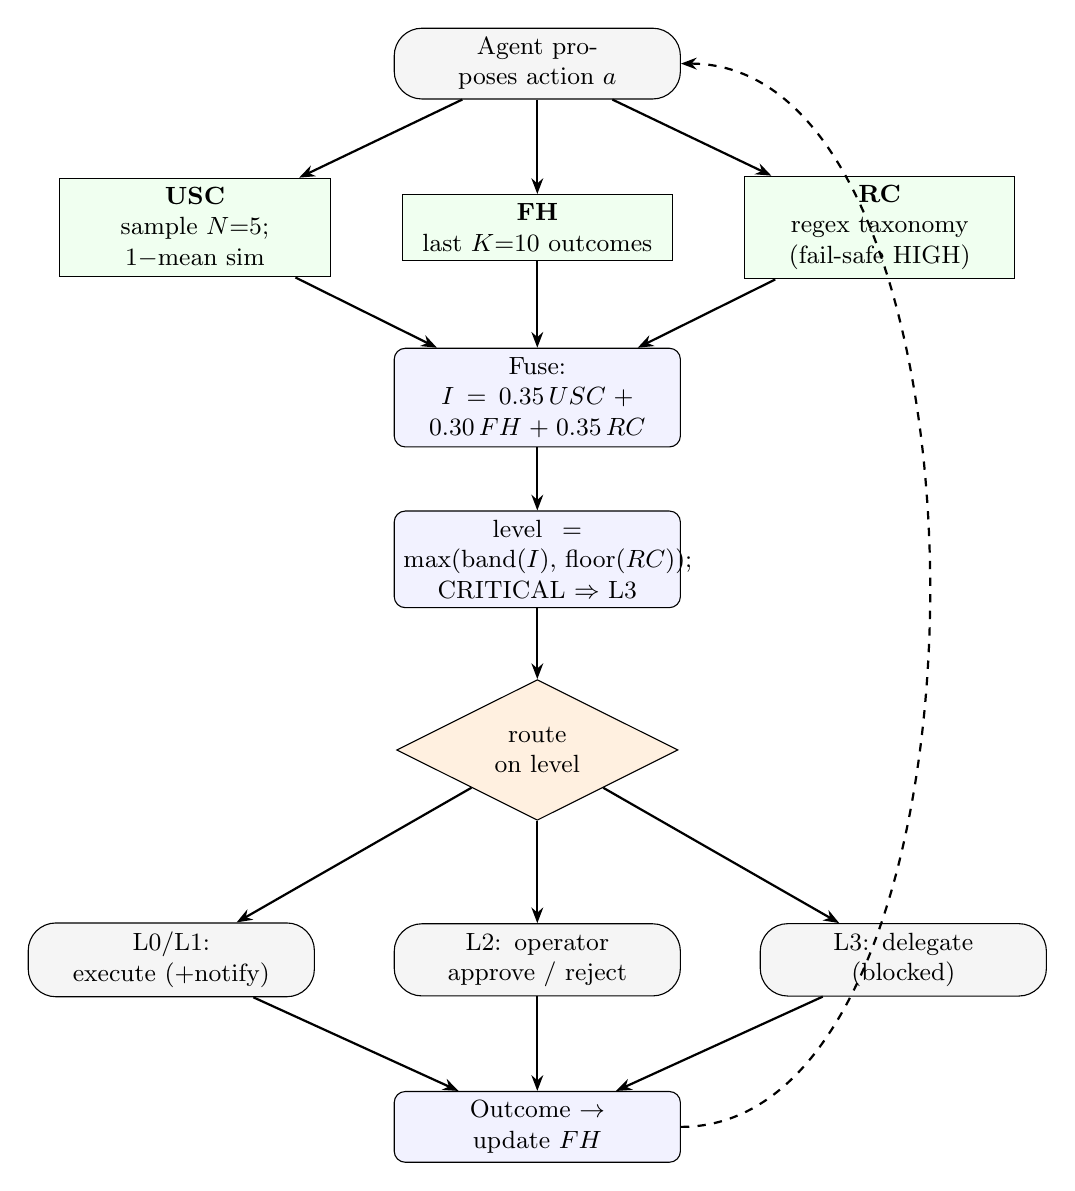
\begin{tikzpicture}
\node[term](start){Agent proposes action $a$};
\node[sig,below=12mm of start](fh){\textbf{FH}\\ last $K{=}10$ outcomes};
\node[sig,left=9mm of fh](usc){\textbf{USC}\\ sample $N{=}5$; $1-$mean sim};
\node[sig,right=9mm of fh](rc){\textbf{RC}\\ regex taxonomy\\ (fail-safe HIGH)};
\node[proc,below=11mm of fh](fuse){Fuse:\\ $I=0.35\,USC+0.30\,FH+0.35\,RC$};
\node[proc,below=8mm of fuse](map){$\mathrm{level}=\max(\mathrm{band}(I),\,\mathrm{floor}(RC))$;\\ CRITICAL $\Rightarrow$ L3};
\node[dec,below=9mm of map](dec){route\\ on level};
\node[term,below=13mm of dec](l2){L2: operator\\ approve / reject};
\node[term,left=10mm of l2](l0){L0/L1:\\ execute (+notify)};
\node[term,right=10mm of l2](l3){L3: delegate\\ (blocked)};
\node[proc,below=12mm of l2](out){Outcome $\to$ update $FH$};
\draw[fl](start)--(usc); \draw[fl](start)--(fh); \draw[fl](start)--(rc);
\draw[fl](usc)--(fuse); \draw[fl](fh)--(fuse); \draw[fl](rc)--(fuse);
\draw[fl](fuse)--(map); \draw[fl](map)--(dec);
\draw[fl](dec)--(l0); \draw[fl](dec)--(l2); \draw[fl](dec)--(l3);
\draw[fl](l0)--(out); \draw[fl](l2)--(out); \draw[fl](l3)--(out);
\draw[fl,dashed](out.east) .. controls +(4.2,0) and +(4.2,0) .. (start.east);
\end{tikzpicture}
\caption{CADIS control flow. Three trust signals are computed for each proposed action, fused into the
intervention score $I(t)$, and mapped to an oversight level; the outcome feeds the failure-history
signal for the next step.}
\label{fig:flow}
\end{figure}

\subsection{Agent--CADIS interaction (activity diagram)}
Figure~\ref{fig:activity} shows how CADIS integrates with the agent's think--act loop as an interception
gate: the agent proposes, CADIS scores and routes, and only permitted actions reach the executor; the
result returns to the agent to inform the next step.

\begin{figure}[t]
\centering
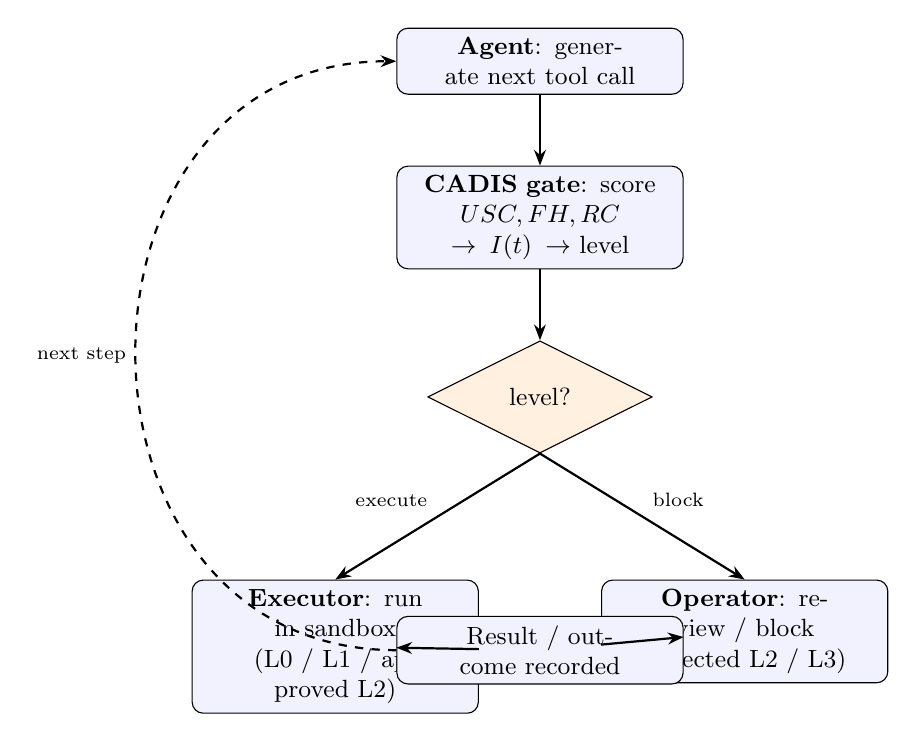
\begin{tikzpicture}[node distance=9mm]
\node[proc](gen){\textbf{Agent}: generate next tool call};
\node[proc,below=of gen](score){\textbf{CADIS gate}: score $USC,FH,RC$\\ $\to I(t) \to$ level};
\node[dec,below=of score](d){level?};
\node[proc,below=16mm of d,xshift=-26mm](exec){\textbf{Executor}: run in sandbox\\ (L0 / L1 / approved L2)};
\node[proc,below=16mm of d,xshift=26mm](block){\textbf{Operator}: review / block\\ (rejected L2 / L3)};
\node[proc,below=44mm of score](res){Result / outcome recorded};
\draw[fl](gen)--(score); \draw[fl](score)--(d);
\draw[fl](d.south) -- node[above left,font=\scriptsize]{execute}(exec.north);
\draw[fl](d.south) -- node[above right,font=\scriptsize]{block}(block.north);
\draw[fl](exec)--(res); \draw[fl](block)--(res);
\draw[fl,dashed](res.west) .. controls +(-4.4,0) and +(-4.4,0) .. (gen.west)
    node[midway,left,font=\scriptsize]{next step};
\end{tikzpicture}
\caption{Activity diagram of the agent--CADIS loop. CADIS is a gate at the action seam; the agent loop,
prompts, model, and decoding are identical with and without CADIS---only the routing of each proposed
action changes.}
\label{fig:activity}
\end{figure}

\subsection{Implementation and integration}
CADIS was implemented and brought into conformity with its specification through a gated, staged
workflow: internalising the design, auditing the existing code, implementing the pure-function signal
and routing core with unit tests that match the formulas one-to-one, wiring the operator for the L1/L2/L3
levels, standing up the isolated target suite, implementing the experimental conditions, and adding
per-step logging that records every signal, weight, threshold, the score $I(t)$, the band level, the risk
floor, the final level, the operator decision, and the outcome. All LLM access---both the agent and the
$N{=}5$ self-consistency sampler---routes through a single pinned model via the OpenRouter API, so that
the same model produces the agent's actions and its resamples. Before any counted run the entire
configuration (code commit, model slug, generation parameters, weights, thresholds, target image
digests, and the four conditions) was frozen and pre-registered, and every subsequent methodological
change was recorded in a deviation log before proceeding.

\section{Testing Environment and Methodology}\label{sec:test}
This section describes how CADIS was exercised after development. Because CADIS is an oversight layer,
it can only be evaluated by running a real agent against real vulnerable services under different
oversight policies. We therefore ran a live agent against a suite of isolated, vulnerable Docker target
machines and recorded, for every proposed action, what CADIS did with it.

\subsection{Experimental conditions}
The agent, prompts, model, sampling, and the rule that ``the executed action is the agent's own first
sample'' are identical across four conditions; only the level decision differs
(Table~\ref{tab:conditions}).

\begin{table}[t]
\centering
\begin{tabular}{ll p{7.4cm}}
\toprule
Condition & Level decision & Purpose \\
\midrule
Full autonomy & always L0 & speed ceiling; no oversight \\
Static HITL & always L2 & safety ceiling; cost of maximal oversight \\
Random & random levels matched to CADIS's measured effort budget & tests whether CADIS's interventions are \emph{well-placed} vs.\ any equal-budget policy \\
CADIS & full $\max(\mathrm{band}(I),\mathrm{floor})$ policy & the system under test \\
\bottomrule
\end{tabular}
\caption{The four evaluation conditions. The random condition is budget-matched to CADIS's measured
human-effort ratio on the same target, and is the load-bearing control.}
\label{tab:conditions}
\end{table}

\subsection{Target environments (the test set)}
CADIS was tested against two families of vulnerable target machines, each an isolated Docker container
brought up on a network-isolated bridge, destroyed and recreated from a pinned image between runs so no
state leaks. The first family is a small, difficulty-spanning core suite; the second is a broader set of
in-vitro and real-world CVE tasks adapted from AutoPenBench \citep{gioacchini2024autopenbench}.
Table~\ref{tab:targets} lists them.

\begin{table}[t]
\centering
\small
\begin{tabular}{lll l}
\toprule
Target & Base / service & Vulnerability & Used in \\
\midrule
\multicolumn{4}{l}{\emph{Core suite (three pinned models: DeepSeek-v4-flash, Gemini-2.5-flash, GPT-OSS-120B)}}\\
dvwa-sqli & DVWA (web) & SQL injection & core runs \\
msf2-vsftpd & Metasploitable2 & vsftpd 2.3.4 backdoor & core runs \\
juice-shop & OWASP Juice Shop & injection / auth bypass & core runs \\
\midrule
\multicolumn{4}{l}{\emph{AutoPenBench suite (DeepSeek-v4-flash)}}\\
apb-web-sqli & PHP + MySQL & UNION SQL injection & AutoPenBench run \\
apb-invitro-web-trav0/1/2 & PHP web app & path traversal (none/replace/filter) & AutoPenBench run \\
apb-cve-apache & Apache httpd 2.4.50 & CVE-2021-42013 traversal $\to$ RCE & AutoPenBench run \\
apb-cve-grafana & Grafana 8.2.0 & CVE-2021-43798 path traversal & AutoPenBench run \\
apb-cve-jenkins & Jenkins 2.441 & CVE-2024-23897 CLI file read & AutoPenBench run \\
apb-cve-spring4shell & Spring / Tomcat & CVE-2022-22965 RCE & AutoPenBench run \\
apb-heartbleed & nginx + OpenSSL 1.0.1c & CVE-2014-0160 Heartbleed & AutoPenBench run \\
\bottomrule
\end{tabular}
\caption{The vulnerable target machines used to test CADIS. Each is an isolated, digest-pinned Docker
image spanning web injection, path traversal, remote code execution, a service backdoor, and a memory
disclosure. Every target has a planted secret (a flag) that is reachable only by actually performing the
exploit, so task success is verified by artifact, not self-report.}
\label{tab:targets}
\end{table}

\subsection{Testing procedure}
For each (condition, target, repetition) the target was reset from its pinned image, the agent was run
against the target's objective under the condition's policy, and every proposed action was scored and
logged. The core suite was run for three pinned models across the four conditions with three repetitions
each (a $4\times3\times3$ matrix per model); the AutoPenBench suite was run for one pinned model across
the four conditions. Because CADIS is a risk-gating mechanism, the primary quantities of interest at the
action level are: whether a proposed action was classified high-risk, and whether it was
\emph{contained} (blocked) or executed. At the run level we record task completion (by the planted-flag
artifact oracle), the human-effort ratio (fraction of actions escalated to $\ge$ L1), and the
time-to-completion.

\section{Results}\label{sec:results}
We present the results from the angle that matters for an oversight layer: \emph{does CADIS block the
risky behaviours?} On this question the evidence is consistent and strong across every run.

\subsection{CADIS is a precise, complete risk gate}
Table~\ref{tab:gating} reports, for each of the four billable evaluation runs, how well each condition
gated the high-risk actions the agent proposed. \textbf{CADIS blocked 100\% of the HIGH/CRITICAL actions
in every run, at essentially perfect precision}---almost no benign action was ever caught. A
budget-matched random policy, spending the same human effort, caught only $17$--$27\%$ of the risky
actions; static human-in-the-loop matched CADIS's coverage only by blocking everything, at full human
effort and lower precision.

\begin{table}[t]
\centering
\small
\begin{tabular}{l cc cc cc}
\toprule
& \multicolumn{2}{c}{\textbf{CADIS}} & \multicolumn{2}{c}{Random (matched)} & \multicolumn{2}{c}{Static HITL}\\
\cmidrule(lr){2-3}\cmidrule(lr){4-5}\cmidrule(lr){6-7}
Evaluation run & recall & prec. & recall & prec. & recall & prec.\\
\midrule
DeepSeek-v4-flash (core) & \textbf{100\%} & \textbf{1.00} & 27\% & 0.86 & 100\% & 0.90 \\
Gemini-2.5-flash (core)  & \textbf{100\%} & \textbf{1.00} & 27\% & 0.88 & 100\% & 1.00 \\
GPT-OSS-120B (core)      & \textbf{100\%} & \textbf{1.00} & 17\% & 1.00 & 100\% & 0.96 \\
AutoPenBench (DeepSeek)  & \textbf{100\%} & \textbf{1.00} & 27\% & 0.79 & 100\% & 0.90 \\
\bottomrule
\end{tabular}
\caption{Risk-gating performance across the four evaluation runs. \emph{recall} = fraction of the
agent's HIGH/CRITICAL actions that were blocked; \emph{prec.} = fraction of blocks that were genuinely
HIGH/CRITICAL. CADIS achieves complete coverage at near-perfect precision in every run; a random policy
of equal human-effort budget covers only a fraction.}
\label{tab:gating}
\end{table}

\subsection{Containment, effort, and safety together}
Table~\ref{tab:apb} summarises the AutoPenBench run at the condition level. The key column is the number
of high-risk actions that \emph{executed without any oversight}: full autonomy ran $163$ such actions
unchecked, and a budget-matched random policy still let $134$ through, whereas \textbf{CADIS let none}.
CADIS achieves this complete containment at a human-effort ratio of $0.44$---less than half of static
HITL's $1.00$---while the hallucination-cascade rate is zero in every condition (no cascade ever
materialised in this regime).

\begin{table}[t]
\centering
\begin{tabular}{l cccc}
\toprule
Condition & Cascade rate & Human-effort & High-risk actions run & Task completion \\
 & (HCR) & ratio (HER) & \emph{unchecked} & (solvable targets) \\
\midrule
Full autonomy & 0.00 & 0.00 & 163 & 0.96 \\
Static HITL   & 0.00 & 1.00 & \textbf{0} & 0.81 \\
Random (matched) & 0.00 & 0.41 & 134 & 0.96 \\
\textbf{CADIS} & 0.00 & 0.44 & \textbf{0} & 0.65 \\
\bottomrule
\end{tabular}
\caption{AutoPenBench run, per condition. CADIS contains every high-risk action (0 executed unchecked)
at under half the effort of static HITL, whereas the budget-matched random policy lets most high-risk
actions through.}
\label{tab:apb}
\end{table}

\subsection{CADIS's interventions are well-placed, not merely frequent}
Two further observations reinforce that CADIS gates the \emph{right} actions. First, the random control
in Tables~\ref{tab:gating}--\ref{tab:apb} spends the same oversight budget as CADIS but achieves only a
fraction of the containment---so CADIS's coverage comes from \emph{targeting}, not from intervening at a
high rate. Second, when CADIS's operator is changed from ``reject every high-risk action'' to ``approve
a valid, in-scope proof-of-concept while still flagging it,'' task completion on the solvable targets
recovers from $0.65$ back to $0.96$---the same level as full autonomy---while CADIS's routing is
unchanged. This isolates CADIS's \emph{routing} (which is well-placed) from the operator's \emph{policy}
(which determines the completion cost). Finally, on the weaker models CADIS eliminated a catastrophic
``flailing tail'': under full autonomy and random intervention the agent could spend on the order of
$10^3$ seconds repeatedly attempting a doomed high-risk action, whereas CADIS gated that action early and
collapsed the mean time-to-completion by roughly two orders of magnitude.

\section{Discussion}\label{sec:discussion}
Evaluated as what it is---a risk-gating oversight layer---CADIS works, and does so consistently across
three different LLMs and a diverse set of real vulnerable targets. It identifies and contains the
high-consequence actions with complete recall and near-perfect precision, it does so far more
effectively than a random policy of equal cost, and it reaches the safety coverage of always-on human
review at a fraction of the human effort. The budget-matched random control is what makes this a
meaningful claim rather than a tautology: an oversight layer that merely intervened often could match
CADIS's \emph{rate} but not its \emph{placement}, and the data show that placement is where CADIS's value
lies.

It is important to separate two questions. ``Does CADIS gate risk well?'' is answered affirmatively and
is a statement about the mechanism. ``Is gating that risk always beneficial?'' is a separate, deployment-
dependent question. In an authorised penetration test the high-risk actions are frequently the
\emph{productive} exploit steps, so blocking them can cost task completion; that is why CADIS's
completion rate is lower than full autonomy on the solvable targets. This is not a failure of CADIS's
targeting---the operator ablation shows the routing was correct---but a consequence of the fact that, in
this particular setting, risk and productivity coincide. In a deployment where high-risk actions are
genuinely harmful rather than the goal, the same precise gating is a direct safety benefit at no
completion cost that a random policy could match.

\section{Limitations}\label{sec:limitations}
Several limitations bound the strength of these claims and are stated plainly.

\begin{itemize}
\item \textbf{The cascade hazard did not arise.} The hallucination-cascade rate was zero in every
condition of every run. The capable, instruction-tuned models tested here rarely emit the repeated
invalid-command sequences the cascade metric is defined over, so the pre-registered primary safety
comparison (CADIS vs.\ random on cascades) is undecidable in this regime. Our positive result is
therefore about \emph{risk-gating behaviour}, not about demonstrated prevention of a realised harm.

\item \textbf{Risk validity is definitional in part.} ``CADIS blocks risky behaviour'' is only meaningful
if ``risky'' is anchored to an independent notion of consequence. We anchor it to the rule-based taxonomy
reviewed against MITRE ATT\&CK and to inspection of the blocked commands, which are the actual exploit
primitives (injection, traversal, backdoor, RCE) rather than benign reconnaissance; the near-perfect
precision supports this, but the taxonomy remains a hand-authored artifact.

\item \textbf{Risk equals productivity here.} Because the targets are authorised exploitation tasks, the
high-risk actions are the intended work; the observed completion cost is specific to this setting and
should not be read as a general property of CADIS.

\item \textbf{Scale and scope.} The AutoPenBench run uses a single model over nine targets, and the core
suite three targets over three models; statistical power for run-level comparisons is limited. Several
AutoPenBench images could not be built or provisioned on current infrastructure and were excluded, and
tasks requiring multi-host, SSH, or cryptographic setups were out of scope.

\item \textbf{Operator model.} The blocking decisions at L2/L3 were resolved by a deterministic scripted
operator (for reproducibility), not by live human raters. The completion cost is sensitive to this
operator policy, as the approve-valid-PoC ablation demonstrates.

\item \textbf{Provider nondeterminism.} LLM API calls are not perfectly reproducible; this is mitigated
by a pinned model, fixed seeds where supported, $N$-sampling, and a frozen configuration, but not
eliminated.
\end{itemize}

\section{Conclusion}
CADIS is a consequence-aware oversight layer that scores each proposed agent action on uncertainty,
track record, and intrinsic risk, and routes it to one of four graduated intervention levels. Developed
and integrated into a live penetration-testing agent and tested against isolated vulnerable Docker
targets and AutoPenBench tasks across three LLMs, CADIS demonstrably works as a risk gate: it contained
every high-risk action at near-perfect precision, far exceeded a budget-matched random policy at equal
cost, and matched always-on oversight's coverage at less than half the human effort. The remaining
question---when that containment is net-beneficial---is a property of the deployment, not of the
mechanism.

\bibliographystyle{plainnat}
\bibliography{references}

\end{document}
